\documentclass[output=paper,colorlinks,citecolor=brown]{langscibook} 
\ChapterDOI{10.5281/zenodo.6393758}
\author{Mohamed Mwamzandi\affiliation{University of North Carolina at Chapel Hill}}
\title{The pragmatics of Swahili relative clauses}
\abstract{Several studies explain the variation of the Swahili relative clause (RC) from a syntactic perspective. These studies discuss the derivational and structural differences/similarities between the \textit{amba} RC and the tensed RC. In this study, the choice between the \textit{amba} and tensed RCs is explained from a pragmatic perspective. 440 RCs were extracted from the Helsinki Corpus of Swahili. The dataset was then coded for various variables including relative marker (\textit{amba}/tensed), relative type (restrictive/non-restrictive), length (number of words used), and information status (topic/non-topic). The results show that the tensed RCs are mostly restrictive while the \textit{amba} RCs are mostly non-restrictive. Further, the mean length of the \textit{amba} RC is higher than of the tensed RC. It was observed that the \textit{amba} RC is preferred in topic shift transition, that is, when a non-topic NP becomes the topic NP in the following utterance while the tensed RC is preferred in continue transition, that is, if the topic of the matrix clause is the same as that of the RC.}
\IfFileExists{../localcommands.tex}{
  \addbibresource{localbibliography.bib}
  \usepackage{langsci-optional,langsci-branding}
\usepackage{langsci-gb4e}
% \usepackage{langsci-textipa}
% \usepackage{langsci-glyphs}
\usepackage[linguistics]{forest}
\usepackage{tabto}
\usepackage{multirow}
\usepackage{bbding}

\usepackage[normalem]{ulem}

\usepackage{tikz-qtree}

\usepackage{enumitem}

\usepackage{multicol}
\usepackage{stmaryrd} %double brackets

\makeatletter
\let\pgfmathModX=\pgfmathMod@
\usepackage{pgfplots,pgfplotstable}%
\let\pgfmathMod@=\pgfmathModX
\makeatother
\usepgfplotslibrary{colorbrewer}
\usetikzlibrary{fit}

\usepackage{jambox}
\usepackage{tikz-qtree-compat}
\usetikzlibrary{arrows, arrows.meta}
\usepackage{longtable}
\usepackage{subcaption}

  \makeatletter
\let\thetitle\@title
\let\theauthor\@author
\makeatother

\newcommand{\togglepaper}[1][0]{
%   \bibliography{../localbibliography}
  \papernote{\scriptsize\normalfont
    \theauthor.
    \thetitle.
    To appear in:
    Change Volume Editor \& in localcommands.tex
    Change volume title in localcommands.tex
    Berlin: Language Science Press. [preliminary page numbering]
  }
  \pagenumbering{roman}
  \setcounter{chapter}{#1}
  \addtocounter{chapter}{-1}
}

\newcommand{\bari}{\ipabar{\i}{.5ex}{1.1}{}{}}
\newcommand{\notipa}[1]{\textnormal{#1}}

\newcommand{\agre}{\textsc{agr}-\ol{eene}}

\renewcommand{\emph}[1]{\textit{#1}} % resetting a setting from ling-macros-modified (I think?)

% forest settings to make compact but (mostly) straight-spined trees:
\forestset{
fairly nice empty nodes/.style={
            delay={where content={}{shape=coordinate,for parent={
                  for children={anchor=north}}}{}}
, angled/.style={content/.expanded={$<$\forestov{content}$>$}}
}}

\forestset{sn edges/.style={for tree={parent anchor=south, child anchor=north}}}

\newcommand{\bex}{\begin{exe}}
\newcommand{\fex}{\end{exe}}

\newcommand{\bxl}{\begin{exe}}
\newcommand{\fxl}{\end{exe}}

\newcommand{\ix}[1]{\textsubscript{#1}}
\newcommand{\alert}[1]{\textbf{#1}}
\newcommand{\ol}[1]{\textit{#1}}


			\usetikzlibrary{shapes,arrows,positioning,decorations,decorations.pathmorphing,intersections}
\forestset{
nice empty nodes/.style={
    for tree={calign=fixed edge angles},
    delay={where content={}{shape=coordinate,for siblings={anchor=north}}{}}
},
}

\definecolor{dark-gray}{gray}{0.3}

%\usepackage{dingbat,pifont}


%%%%%%%%%%%%For arrows%%%%%%%%%%%%%

\newcommand\Tikzmark[2]{%
  \tikz[remember picture]\node[inner sep=0pt,outer sep=0pt] (#1) {#2};%
}
\NewDocumentCommand\DrawArrow{O{}mmmmO{3}}{
\tikz[remember picture,overlay]
  \draw[->,line width=0.8pt,shorten >= 2pt,shorten <= 2pt,#1]
    (#2) -- ++(0,-#6\ht\strutbox) coordinate (aux) -- node[#4] {#5} (#3|-aux) -- (#3);
}
\NewDocumentCommand\DrawDotted{O{}mmmmO{3}}{
\tikz[remember picture,overlay]
  \draw[->,line width=0.9pt,dotted,shorten >= 2pt,shorten <= 2pt,#1]
    (#2) -- ++(0,-#6\ht\strutbox) coordinate (aux) -- node[#4] {#5} (#3|-aux) -- (#3);
}
\NewDocumentCommand\DrawLine{O{}mmmmO{3}}{
\tikz[remember picture,overlay]
  \draw[line width=0.8pt,shorten >= 2pt,shorten <= 2pt,#1]
    (#2) -- ++(0,-#6\ht\strutbox) coordinate (aux) -- node[#4] {#5} (#3|-aux) -- (#3);
}
%%%%%%%%%%%%%%%%%%%%%%%%%%%%%%%%%%%%%


\newcommand{\baru}{ʉ}
\newcommand{\baruH}{\'\baru}
\newcommand{\baruL}{\`\baru}

\newcommand{\ep}{ε}
\newcommand{\epH}{\'\ep}
\newcommand{\epL}{\`\ep}

\newcommand{\schwa}{ə}
\newcommand{\schwaH}{\'ə}
\newcommand{\schwaL}{\`ə}

\newcommand{\oo}{ɔ}
\newcommand{\ooH}{\'\oo}
\newcommand{\ooL}{\`\oo}

\newcommand{\ds}{\textsuperscript{
	\hspace*{-2pt}\begin{tikzpicture}
		\draw[-{>[scale=0.5]}] (0,0.4) --(0,0.25);
	\end{tikzpicture}}}

\newcommand{\ch}{t͡ʃ}
\newcommand{\dz}{d͡ʒ}

\newcommand{\tgl}{ʔ}

%shortcuts for the complementizers
\newcommand{\mbuL}{mb\baruL}
\newcommand{\mbuHL}{mb\baruH\baruL}
\newcommand{\mbuLH}{mb\baruL\baruH}
\newcommand{\la}{lá}
\newcommand{\nda}{ndà}

\newcommand{\tsc}[1]{\textsc{#1}}
\renewcommand{\textscb}{ʙ}
\newcommand{\ipa}[1]{#1} %disable IPA

\newcommand{\SM}[1]{#1}

\DeclareNewSectionCommand
  [
    counterwithin = chapter,
    afterskip = 2.3ex plus .2ex,
    beforeskip = -3.5ex plus -1ex minus -.2ex,
    indent = 0pt,
    font = \usekomafont{section},
    level = 1,
    tocindent = 1.5em,
    toclevel = 1,
    tocnumwidth = 2.3em,
    tocstyle = section,
    style = section
  ]
  {appendixsection}

\renewcommand*\theappendixsection{\Alph{appendixsection}}
\renewcommand*{\appendixsectionformat}
              {\appendixname~\theappendixsection\autodot\enskip}
\renewcommand*{\appendixsectionmarkformat}
              {\appendixname~\theappendixsection\autodot\enskip}

\renewcommand{\lsChapterFooterSize}{\footnotesize}
 
  %% hyphenation points for line breaks
%% Normally, automatic hyphenation in LaTeX is very good
%% If a word is mis-hyphenated, add it to this file
%%
%% add information to TeX file before \begin{document} with:
%% %% hyphenation points for line breaks
%% Normally, automatic hyphenation in LaTeX is very good
%% If a word is mis-hyphenated, add it to this file
%%
%% add information to TeX file before \begin{document} with:
%% %% hyphenation points for line breaks
%% Normally, automatic hyphenation in LaTeX is very good
%% If a word is mis-hyphenated, add it to this file
%%
%% add information to TeX file before \begin{document} with:
%% \include{localhyphenation}
\hyphenation{
affri-ca-te
affri-ca-tes 
Līk-pāk-páln
pro-sod-ic
phe-nom-e-non
Chi-che-wa
Lu-bu-ku-su
Ngbu-gu
Boyel-dieu
Mat-chi
pho-neme
Mil-em-be
Nyan-chera
Mc-Pher-son
Tsoo-tso
Sku-pin
dis-tin-guishes
con-ser-va-tion
Me-dum-ba
}

\hyphenation{
affri-ca-te
affri-ca-tes 
Līk-pāk-páln
pro-sod-ic
phe-nom-e-non
Chi-che-wa
Lu-bu-ku-su
Ngbu-gu
Boyel-dieu
Mat-chi
pho-neme
Mil-em-be
Nyan-chera
Mc-Pher-son
Tsoo-tso
Sku-pin
dis-tin-guishes
con-ser-va-tion
Me-dum-ba
}

\hyphenation{
affri-ca-te
affri-ca-tes 
Līk-pāk-páln
pro-sod-ic
phe-nom-e-non
Chi-che-wa
Lu-bu-ku-su
Ngbu-gu
Boyel-dieu
Mat-chi
pho-neme
Mil-em-be
Nyan-chera
Mc-Pher-son
Tsoo-tso
Sku-pin
dis-tin-guishes
con-ser-va-tion
Me-dum-ba
}
 
  \togglepaper[1]%%chapternumber
}{}

\begin{document}
\SetupAffiliations{mark style=none}
\maketitle 

\section{Introduction}\label{sec:mwamzandi:1}

Several studies discuss the syntax of the Swahili tensed relative marker (RM) \REF{ex:mwamzandi:1} and the \textit{amba} RM \REF{ex:mwamzandi:2}. The goal of these studies is to draw a parallel between the two by explaining how the position of the RM is derivable from the same underlying position (\citealt{Vitale1981, Keach1985}) or occupies the same syntactic position (\citealt{DemuthHarford1999, Ngonyani2001, Ngonyani2006}). The examples presented in this study are from the Helsinki Corpus of Swahili (written texts in the standard Swahili), otherwise, citation will be given. The following notational conventions are followed: the RM is glossed as SRM (subject RM) or ORM (object RM) and the RC is bracketed.

\ea%1
    \label{ex:mwamzandi:1}
    \gll    Askari [a-li-ye-ki-ongoza kikosi].\\
            1.policeman  \textsc{1.sm-pst-1.srm-7.om-}lead  7.squad]\\
    \glt    ‘The policeman who led the squad.’
\ex%2
    \label{ex:mwamzandi:2}
    \gll    Askari [amba-ye a-li-ki-ongoza kikosi].\\
            1.policeman  amba\textsc{-1.srm}  \textsc{1.sm-pst-7.om-}lead  7.squad\\
    \glt    ‘The policeman who led the squad.’
\z

In \REF{ex:mwamzandi:1} the SRM \textit{ye-}, which agrees with the head noun \textit{askari} ‘policeman’ in number and noun class is prefixed to the verb after tense while in \REF{ex:mwamzandi:2} it is suffixed to \textit{amba}. In Swahili and other Bantu languages, a predicate has a subject marker prefix that agrees with the subject in number and noun class and may also carry an object marker prefix. In \REF{ex:mwamzandi:1}, the subject marker prefix \textit{a-} occurring in the verb initial position corresponds to the noun class 1 NP \textit{askari} ‘police’ while the object marker prefix \textit{ki-} occurring after the SRM \textit{ye-} in \REF{ex:mwamzandi:1} and after the tense marker \textit{li-} in \REF{ex:mwamzandi:2} corresponds to the noun class 7 NP \textit{kikosi} ‘squad’. I should mention that there is yet another type of RM referred to as the general relative exemplified in \REF{ex:mwamzandi:3}.

\ea%3
    \label{ex:mwamzandi:3}
    \gll    Askari a-ki-ongoz-a-ye kikosi.\\
            1.policeman  \textsc{1.sm-7.om-}lead\textsc{-fv-1.srm}  squad\\
    \glt    ‘The policeman who is leading the squad.’
\z

The SRM \textit{-ye} in \REF{ex:mwamzandi:3} is suffixed to the verb after the final vowel. Time is unspecified in the general relative and it is used in cases interpreted as present or habitual \citep{Ashton1944}. In this study, I explain the variation of the tensed RC and the \textit{amba} RC from a pragmatic perspective and leave the general relative for future research. “Pragmatics” is defined as “the systematic study of meaning by virtue of, or dependent on, the use of language” \citep[2]{Huang2007}. Notice that the tensed and the \textit{amba} relative clause in \REF{ex:mwamzandi:1} and \REF{ex:mwamzandi:2} are grammatical and are truth conditionally equivalent. The aim of this study is to give a pragmatic account of the variation. I should mention that most of the explanations for the variation of the Swahili \textit{amba} and tensed RCs in this study are not absolute but statistical tendencies and should be considered in their entirety rather than individually.

Based on a few selected examples from texts, earlier studies have made claims that the \textit{amba} RM is required in non-restrictive RCs, but this is yet to be confirmed using a large dataset (\citealt{Ashton1944, Schadeberg1989}). A restrictive RC as illustrated in \REF{ex:mwamzandi:5} delimits the referent of an NP \citep[206]{Andrews2007}. On the other hand, a non-restrictive RC as illustrated in \REF{ex:mwamzandi:4} makes a comment about an NP or another constituent without delimiting its referent. 

\ea%4
    \label{ex:mwamzandi:4}
    The Japanese [who/that are industrious] now outcompete Europe.
\ex%5
    \label{ex:mwamzandi:5}
    The Japanese, [who/(*that) are industrious], now outcompete Europe. \hfill \citep[168]{Keenan1985}
\z

In English, the restrictive clause in \REF{ex:mwamzandi:4} allows the occurrence of the complementizer \textit{that} but the non-restrictive clause in \REF{ex:mwamzandi:5} does not. It is also possible to suppress the relative pronoun in a restrictive RC as in: \textit{The man I saw yesterday left this morning}, but not in a non-restrictive RC \citep[139]{Comrie1989}. Further, as indicated by the comma before and after the RC, the non-restrictive clause as seen in \REF{ex:mwamzandi:5} is set off intonationally from the main clause. Although the dataset in this study shows that the \textit{amba} relative is mostly used in non-restrictive RCs, both the tensed and \textit{amba} RCs can be used restrictively as well as non-restrictively. Thus, the restrictive and non-restrictive variable alone may not explain the Swahili \textit{amba} and tensed RC variation. In addition to being used in non-restrictive RCs, it has been claimed that the \textit{amba} RC when contrasted with the tensed RC is morphologically more versatile; its word order more flexible; and its structure more complex (\citealt{Schadeberg1989, Russell1992}).

I explore via corpus analysis the following questions:
 
\begin{enumerate}
        \item The frequency of use of the \textit{amba} RC and tensed RC as restrictive/non-restrictive and its implications in the variation.
        \item Whether the speaker’s choice of the \textit{amba}\slash tensed RC is influenced by the length of the RC measured in number of words.
\end{enumerate}
I should mention that cross-linguistic studies have mostly analyzed complexity of RCs resulting from movement, locality, intervention and feature similarity as well as word order expectation (see, for example, \citealt{DurrlemanEtAl2016, Rizzi2013Locality, LevyEtAl2013}). Because of the difficulty in measuring complexity in written texts whose verification needs processing tests performed on speakers, this study investigates the effect of RC length on the Swahili \textit{amba} and tensed RC variation. It is assumed that longer sentences have more phrases, clauses and optional adjuncts that require subordination and coordination (cf. \citealt{HemforthEtAl2015}, who investigate the effect of length on high attachment (first noun modification) and low attachment (second noun modification) in the processing of relative clauses with two possible antecedents in English, Spanish and French). 

\begin{enumerate}
        \item[3.] Whether the grammatical role (subject/object) of the head noun in the matrix clause and information status of the head NP, specifically topic, impacts on the type of RC used. 
\end{enumerate}
There are some parameters that may help in identifying the topic in an utterance. These include grammatical role, pronominalization, and linear order of discourse entities. I posit that the notion of topic, defined as what the proposition is about (\citealt{Gundel1985, Lambrecht1994}), play a role on the choice of one form of the RCs over the other. Subjects are mostly topics while objects may be part of a comment in a topic-comment utterance structure. Based on qualitative and quantitative analysis of the dataset, I claim that the \textit{amba} RC is preferred if an NP in a previous utterance is the topic of the RC in a shift transition while the tensed relative is preferred if the most salient NP (topic) of the matrix clause is also the topic of the RC.

The rest of the paper is organized as follows. In \sectref{sec:mwamzandi:2} I discuss previous work that explains the variation of the Swahili \textit{amba} and tensed RCs. In \sectref{sec:mwamzandi:3} I briefly explain the methodology. I present the results of the study and discussion in \sectref{sec:mwamzandi:4} followed by the conclusion in \sectref{sec:mwamzandi:5}.

\section{Previous studies on the Swahili RC variation}\label{sec:mwamzandi:2}

The Swahili RC variation have mostly been attributed to morphosyntactic restrictions on the tensed RM. While the \textit{amba} RM may be used with all the tense, aspect and modality (TAM) markers, the tensed RC may only be used with the past tense marker \textit{li,} present tense marker \textit{na}, the future tense marker \textit{taka}, and the \textit{si} negation marker (see \citealt{Keach1985} for a detailed description of TAM markers that require the use of \textit{amba}). Due to the verb status of the tense markers and \textit{amba} from a diachronic perspective, it has been argued that the two Swahili RCs are structurally the same (\citealt{Vitale1981, Keach1985, DemuthHarford1999, Ngonyani2001, Ngonyani2006}). A subject postposing rule in object RCs have been used as evidence to argue for the same syntactic position of the Swahili RM. Example \REF{ex:mwamzandi:6} and \REF{ex:mwamzandi:7} show the \textit{amba} and tensed object RC respectively.

\ea%6
    \label{ex:mwamzandi:6}
    \gll    Kikosi [amba-cho Kisaka a-li-ki-ongoza].\\
            squad  amba\textsc{-7.orm}  1.Kisaka  \textsc{1.sm-pst-7.om-}lead\\
    \glt    ‘The squad which Kisaka led.’
\ex%7
    \label{ex:mwamzandi:7}
    \gll    Kikosi  [a-li-cho-ki-ongoza Kisaka].\\
            7.squad  \textsc{1.sm-pst-7.orm-7.om-}lead  1.Kisaka\\
    \glt    ‘The squad which Kisaka led.’
\z

The prefix \textit{a} attached to the verb \textit{ongoza} ‘lead’ corresponding to the noun class 1 NP indicates that \textit{kisaka} is the subject of the RC while the RM \textit{cho} corresponding to the noun class 7 NP \textit{kikosi} indicates that the object NP marked by the prefix \textit{ki} before the root of the verb is the relativized NP. In \REF{ex:mwamzandi:6} the subject, \textit{kisaka,} is preverbal but postverbal in \REF{ex:mwamzandi:7}. Notice that the head noun \textit{kikosi} ‘squad’ occurs before \textit{amba/}tense (\textit{li}). \citet{Keach1985} argues that the tensed RM and the \textit{amba} RM are both independent words (verbs) and that nothing can intervene between the head noun and \textit{amba}/tense, hence, the postverbal position of the subject in the tensed object RC in \REF{ex:mwamzandi:7}. However, the structural similarities/differences may not explain why one of the RCs may be chosen instead of the other in discourse texts. 

\citet[125--126]{Russell1992} argues that \textit{amba} is used in object RCs to disambiguate the subject and object NPs if they both belong to the same noun class as illustrated in \REF{ex:mwamzandi:8} and \REF{ex:mwamzandi:9}.

\ea%8
    \label{ex:mwamzandi:8}
    \gll    Mwivi [a-li-ye-mw-ona mtoto].\\
            1.thief  \textsc{1.sm-pst-1.rm-1.om-}see  1.child\\
    \glt    ‘The thief who saw the child/The thief whom the child saw.’
\ex%9
    \label{ex:mwamzandi:9}
    \gll    Mwivi [amba-ye mtoto a-li-mw-ona].\\
            1.thief  amba\textsc{-1.orm} 1.child \textsc{1.sm-pst-1.om-}see\\
    \glt    ‘The thief whom the child saw.’
\z

The NPs \textit{mwivi} ‘thief’ and \textit{mtoto} ‘child’ agree in number and class with the verb \textit{a-li-mu-ona} and can therefore be both interpreted as subject/object in \REF{ex:mwamzandi:8} since Swahili allows both the SVO and OVS word order. The use of \textit{amba} licenses the occurrence of the subject in its canonical preverbal position as seen in \REF{ex:mwamzandi:9} and therefore enhances the interpretation of \textit{mtoto} ‘child’ as the subject of the RC. However, the disambiguation justification for the choice of \textit{amba} is limited in its application since cross-reference can establish the subject and object grammatical roles in situations where the two belong to different noun classes as seen in \REF{ex:mwamzandi:10}.

\ea%10
    \label{ex:mwamzandi:10}
    \gll    Mwivi wa-li-ye-mu-ona watoto.\\
            1.thief  \textsc{2.sm-pst-1.orm-1.om-}see 2.children\\
    \glt    ‘The thief who the children saw.’
\z

In \REF{ex:mwamzandi:10}, the subject of the RC is \textit{watoto} ‘children’ because the subject marker \textit{wa} on the verb agrees with the noun class 2 NP \textit{watoto} ‘children’. Furthermore, as was mentioned by an anonymous reviewer, although \textit{amba} is used in \REF{ex:mwamzandi:11} the subject of the sentence remains ambiguous if the NP \textit{mtoto} ‘child’ occurs after the verb.

\ea%11
    \label{ex:mwamzandi:11}
    \gll    Mwivi [amba-ye a-li-mw-ona mtoto].\\
            1.thief  amba\textsc{-1.orm} \textsc{1.sm-pst-}see 1.child\\
    \glt    ‘The thief whom the child saw.’
\z

Considering examples such as \REF{ex:mwamzandi:10} and \REF{ex:mwamzandi:11}, the choice of the \textit{amba} relative may not be necessarily to disambiguate the subject/object grammatical roles. Furthermore, the grammatical role (subject/object) and function (agent/theme) of discourse entities belonging to the same/different noun classes can be identified if adequate contextual background is available. In texts, discourse entities are linked via referring expression and therefore parameters such as linear order of utterances, subjecthood and pronominalization can help identify the intended referents as well as their grammatical role and information statuses (cf. \citealt{GroszEtAl1995} and \citeauthor{GroszSidner1998}'s \citeyear{GroszSidner1998} Centering Theory, which attempts to determine topic in discourse texts).

In Swahili, it has been claimed that the \textit{amba} RC is preferred if the RC in question is complex as illustrated in \REF{ex:mwamzandi:12} and \REF{ex:mwamzandi:13}.

\ea%12
    \label{ex:mwamzandi:12}
    \gll    Masanduku  [amba-yo sisi watu wa-wili au wa-tatu ha-tu-wez-i]\textsubscript{1} [ku-ya-enua]\textsubscript{2}.\\
            6.boxes  amba\textsc{-6.orm} us 2.people \textsc{2.agr-}two or \textsc{2.agr-}three  \textsc{neg-1pl-}able\textsc{-sbjv} \textsc{inf-6.om-}lift\\
    \glt    ‘Boxes which two or three of us cannot lift.’
\ex%13
    \label{ex:mwamzandi:13}
    \gll    Masanduku [tu-si-yo-weza sisi watu wa-wili au watatu] ku-ya-enua]\textsubscript{2}.\\
            6.boxes  \textsc{1.pl-neg-6.orm-}able us 2.people \textsc{2.agr-}two or \textsc{2.agr-}three \textsc{inf-6.om-}lift\\
    \glt    ‘Boxes which two or three of us cannot lift.’ \hfill \citep[310]{Ashton1944}
\z

Following \citegen{KeenanComrie1977} Accessibility Hierarchy of relativization, it has been claimed that the \textit{amba} RC in \REF{ex:mwamzandi:12} is preferred  instead of the tensed RC in \REF{ex:mwamzandi:13} since the relativized NP is the object (which is higher in the Accessibility Hierarchy than the subject). Based on the dataset used in this study, I argue that the choice of the \textit{amba} RM in \REF{ex:mwamzandi:12} is influenced by the length of the RC rather than the position of the head noun in the Accessibility Hierarchy. Notice that the RC in \REF{ex:mwamzandi:12} contains two clauses with 8 words. The \textit{amba} relative clause may be used by the speaker to “compensate for (perceived) difficulties in producing or parsing” long relative clauses, whether subject or object RCs \citep[133]{Green1996}.

In these syntactic studies on Swahili RC, the structural differences/similarities are the focus and their usage by speakers is regarded as a case of free variation. However, a combination of pragmatic factors such as preference for the tensed RC in restrictive RCs, length of the RCs, and information structure considerations may better explain the choice of one of the RC variants in natural language.

\section{Methodology}\label{sec:mwamzandi:3}

The source of data in this study was the Helsinki Corpus of Swahili (HCS) which has 25 million words. The corpus contains Swahili newspaper articles as well as excerpts of literary texts, education and science material written from the mid-20\textsuperscript{th} century to 2015. In the HCS, concordance searches are done via an inbuilt software, namely \textit{Korp}. \textit{Korp} displays a concordance list of the query as well as the immediate context of the search expression. Every word in the Helsinki corpus contains information related to its parts of speech (for example; verb, noun, adjective), morphological description (for example, relative marker, reciprocal, tense), syntactic function (for example; subject, main verb, object), and gloss in English. The tensed RCs were displayed using an extended search that instructed \textit{Korp} to look for words whose parts of speech was V (verb) and its morphology included REL (relative marker). The \textit{amba} RCs were displayed using a search that queried for all occurrences with \textit{amba} as the base form. Only TAM markers that allow the occurrence of both the \textit{amba} and tensed RCs were selected. Further, the RCs were selected such that they represent the diverse sources in the corpus which include novels by different authors, newspapers, and academic articles on literary works. In total, 440 RCs were selected from the HCS; 285 were tensed RCs and 155 were \textit{amba} RCs.

Recall that \textit{Korp} displays the target utterances in their immediate context. The utterances that occur within the context of the target RC provide contextual clues that help in the pragmatic analysis of the Swahili RC variation. Each of the 440 RCs was coded as restrictive or non-restrictive. As explained earlier, a restrictive relative gives specific information that delimit a referent while a non-restrictive clause gives more information (non-identifying) about a referent. The number of words within each RC was then counted to measure its length. After identifying the discourse entities in the target utterance and those occurring before and after it the RC was coded for relativization (subject/object), the grammatical role of the head noun in relation to the matrix clause (subjet/object/PP compliment) and information status of the head NP (topic/non-topic).

\section{Results and discussion}\label{sec:mwamzandi:4}

The study aimed at investigating pragmatic reasons for the variation of Swahili \textit{amba} and tensed RCs. I discuss the results in the following order. In \sectref{sec:mwamzandi:4.1}, I discuss the role of restrictive/non-restrictive on the \textit{amba} RC and tensed RC variation. In \sectref{sec:mwamzandi:4.2}, I discuss the effect of the RC length on the choice of the \textit{amba}/tensed RC. In \sectref{sec:mwamzandi:4.3} I show that information structure, hitherto unexplored, may also impact on the Swahili RC variation.

\subsection{Variation due to restrictive/non-restrictive use of RCs}\label{sec:mwamzandi:4.1}

If the variation of the \textit{amba} and tensed RCs is due to the restrictive and non-restive use of the RCs, I expect the dataset used in the study to have a higher frequency of \textit{amba} non-restrictive RCs than the tensed non-restrictive RCs. On the other hand, I expect a higher frequency of tensed restrictive RCs than \textit{amba} restrictive RCs. Of the 155 \textit{amba} RCs, 32 were restrictive and 123 were non-restrictive. As for the 285 tensed RCs, 245 were restrictive and 40 were non-restrictive. \figref{fig:mwamzandi:1} summarizes these results.

\begin{figure}
% % % 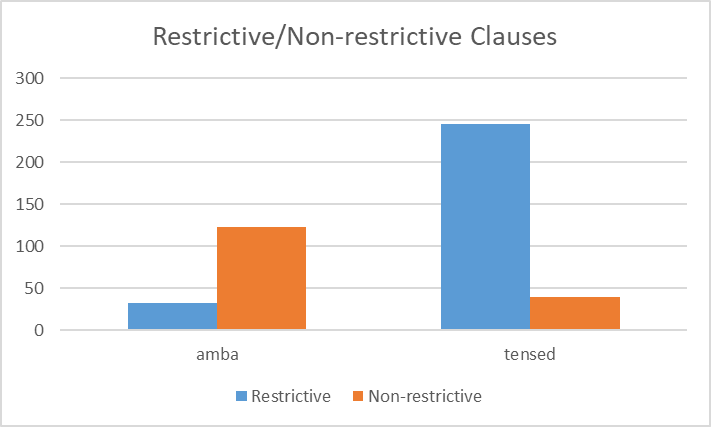
\includegraphics[width=\textwidth]{figures/MwamzandiFig1.png}
    \begin{tikzpicture}
      \begin{axis}[
       ybar,
       axis lines*=left,
       symbolic x coords = {amba,tensed},
       xtick = data,
       nodes near coords,
       enlarge x limits=1,
       bar width=5ex,
       legend pos=outer north east,
       legend cell align=left,
       height=5cm,
       width=8cm
          ]
      \addplot[lsLightOrange,fill=lsLightOrange!20!white,mark=none] coordinates {(amba,32) (tensed,245)};
      \addplot[\lsSeriesColor,fill=\lsSeriesColor!20!white,mark=none] coordinates {(amba,123) (tensed,40)};
      \legend{Restrictive,Non-restrictive}
      \end{axis}
    \end{tikzpicture}
    \caption{\textit{amba} and tensed restrictive and non-restrictive clauses}
    \label{fig:mwamzandi:1}
\end{figure}

A chi-squared test shows that the frequency differences between the restrictive and non-restrictive clauses for the \textit{amba} and tensed RCs is significant $\chi^2 (1,\allowbreak N=440) = 180.89, p < 0.001$. The implication is that the tensed RC is used more frequently as restrictive while the \textit{amba} RC is used more frequently as non-restrictive. I present an example of a tensed restrictive RC in \REF{ex:mwamzandi:14}.

\ea%14
    \label{ex:mwamzandi:14}
    \gll    Bwana yule [a-na-ye-sinzia].\\
            1.man  that  \textsc{1.sm-prs-1.srm-}doze\\
    \glt    ‘That man (over there) who is dozing.’
\z

In \REF{ex:mwamzandi:14}, the speaker points at a specific man who was dozing amongst other men. The RC gives information that help in delimiting the referent of the referring expression \textit{bwana yule} ‘that man’. Although the tensed RC was mostly used restrictively, there are a few instances of tensed non-restrictive RCs illustrated in \REF{ex:mwamzandi:15}.

\ea%15
    \label{ex:mwamzandi:15}
    \gll    A-li-m-rud-i-a Adili [a-li-ye-kuwa a-na-pata fahamu].\\
            \textsc{1.sm-pst-1.om-}return\textsc{-appl-fv} 1.Adili \textsc{1.sm-pst-1.srm-aux} \textsc{1.sm-prs-}get 9.consciousness\\
    \glt    ‘He got back to Adili, who was regaining his consciousness.’
\z

The RC in \REF{ex:mwamzandi:15} does not delimit the referent but gives more information about the topic of the RC, \textit{Adili}. A close analysis of the non-restrictive tensed RCs shows that they mostly occur if the referent of the head noun is a proper noun as is the case in \REF{ex:mwamzandi:15}. There are also cases when a non-restrictive tensed RC gives more information that establishes the identity of a proper noun, as seen in \REF{ex:mwamzandi:16}.

\ea%16
    \label{ex:mwamzandi:16}
    \gll    Krapf [a-li-ye-li-tumikia dhehebu la C.M.S].\\
            Krapf  \textsc{1.sm-pst-1.srm-5.om-}serve 5.denomination of C.M.S.]\\
    \glt    ‘Krapf, who served the C.M.S Christian denomination.’
\z

In \REF{ex:mwamzandi:16}, the head noun \textit{Krapf} is the subject of the RC. The RC presents more specific information that may assist the hearer identify the intended referent.

While the dataset shows that the tensed RC mostly gives information that delimits the referent in restrictive RCs or gives identifying information in non-restrictive usage, the \textit{amba} RC adds new non-identifying information predicated on the head noun as seen in \REF{ex:mwamzandi:17}.

\ea%17
    \label{ex:mwamzandi:17}
    \gll    A-li-kuwa a-me-va-li-a rubega nyeupe [amba-yo i-li-anza ku-poteza weupe wake].\\
            \textsc{1.sm-pst-aux} \textsc{1.sm-pfv-}wear\textsc{-appl-fv} 9.cloak white amba\textsc{-9.srm} \textsc{9.sm-pst-}start \textsc{inf-}loose whiteness its\\
    \glt    ‘He was wearing a white cloak that had started to lose its whiteness.’
\z

In \REF{ex:mwamzandi:17}, the RC gives more information about the head noun, \textit{rubega nyeupe} ‘white cloak’, whose whiteness had faded. The RC in \REF{ex:mwamzandi:16} may be analyzed as an utterance with a topic-comment structure rather than an NP in a coreferential relationship with its antecedent. Although the \textit{amba} RC is mostly non-restrictive, there are instances when the \textit{amba} RC may be used restrictively as seen in \REF{ex:mwamzandi:18}.

\ea%18
    \label{ex:mwamzandi:18}
    \gll    Mambo muhimu [[amba-yo  ya-na-fanya]\textsubscript{1} [shairi li-it-w-e la Ki-swahili]\textsubscript{2}].\\
            6.things important amba\textsc{-6.srm} \textsc{6.sm-prs-}make 6.poem  \textsc{6.sm-}call\textsc{-pass-sbjv} of 7-Swahili\\
    \glt    ‘Important things that make a poem be called a Swahili poem.’
\z

In \REF{ex:mwamzandi:18} the \textit{amba} RC is restrictive because the head noun \textit{mambo muhimu} ‘important things’ are defined by the RC as a set of characteristics that make a poem be called a Swahili poem. Notice that compared to the tensed restrictive clause presented in \REF{ex:mwamzandi:14}, the \textit{amba} restrictive clause in \REF{ex:mwamzandi:18} is longer. The tensed RC is one-word long (one clause) while the \textit{amba} RC is six-words long (two clauses) and both are restrictive and subject RCs. I present the results of the effect of length on Swahili RC variation in \sectref{sec:mwamzandi:4.2}.

\subsection{Length of the relative clause}\label{sec:mwamzandi:4.2}

In this section, I discuss the effect of the RC length measured in number of words on Swahili \textit{amba} RC and tensed RC variation. I claim that the \textit{amba} RC is more frequently used if the length of the RC is long, while the tensed relative is used more frequently in short RCs as illustrated in \REF{ex:mwamzandi:19} and \REF{ex:mwamzandi:20}.

\ea%19
    \label{ex:mwamzandi:19}
    \ea%19a
    \label{ex:mwamzandi:19a}
    \gll    Mwanamke mjane amba-ye a-li-kuwa jirani yao.\\
            1.woman 1.widow amba\textsc{-1.srm} \textsc{1.sm-pst-}be 1.neighbor their\\
    \glt    ‘A (woman) widow who was their neighbor.’
    \ex%19b
    \label{ex:mwamzandi:19b}
    \gll    Mwanamke mjane a-li-ye-kuwa jirani yao.\\
            1.woman  1.widow  \textsc{1.sm-pst-1.srm-}be 1.neighbor their\\
    \glt    ‘A (woman) widow who was their neighbor.’
    \z
\ex%20
    \label{ex:mwamzandi:20}
    \ea%20a
    \label{ex:mwamzandi:20a}
    \gll    Mwanamke mjane amba-ye a-li-kuwa jirani yao hapo zamani.\\
            1.woman  1.widow  amba\textsc{-1.srm} \textsc{1.sm-pst-}be 1.neighbor their long ago\\
    \glt    ‘A (woman) widow who was their neighbor long ago.’
    \ex%20b
    \label{ex:mwamzandi:20b}
    \gll    Mwanamke mjane a-li-ye-kuwa jirani yao hapo zamani.\\
            1.woman 1.widow \textsc{1.sm-pst-1.srm-}be 1.neighbor their long ago\\
    \glt    ‘A (woman) widow who was their neighbor long ago.’
    \z
\z

The RCs in (\ref{ex:mwamzandi:19a}--b) are shorter than the RCs in (\ref{ex:mwamzandi:20a}--b) because of the addition of the adverbial phrase \textit{hapo zamani} in the later. Regardless of the grammatical role of the head noun, the dataset indicates that the \textit{amba} RC was mostly used in cases where the length of the RC in question was long as seen in \REF{ex:mwamzandi:20}. I claim that the \textit{amba} relative is used more frequently in such cases due to its simplifying effect in parsing or producing long RCs.

\tabref{tab:mwamzandi:1} presents the mean and standard deviation (in parenthesis) of the length of the \textit{amba} RCs and tensed RCs (restrictive and non-restrictive).

\begin{table}
    \begin{tabularx}{.55\textwidth}{Xrrrr} 
    \lsptoprule
    & \multicolumn{2}{l}{Restrictive} & \multicolumn{2}{l}{Non-restrictive}\\
    \midrule
    \textit{amba} & 6.34 & (3.25) & 7.21 & (3.71)\\
    tensed & 3.09 & (2.34) & 4.25 & (2.61)\\
    \lspbottomrule
    \end{tabularx}
    \caption{Mean and sd of RC length in restrictive and non-restrictive clauses}
    \label{tab:mwamzandi:1}
\end{table}

The mean length of the \textit{amba} RCs is higher (about 7 words) than that of the tensed RCs (about 4 words). A non-repeated measures ANOVA with RC length as the independent variable, and RM (\textit{amba}/tensed) and relative type (restrictive\slash non-restrictive) as the dependent variables reveal that there is a significant main effect of RC length on RM, $(1,440)=197.49, p<0.001$, and relative type $F(1,440)=11.11, p<0.001$. These results indicate that the \textit{amba} RC is preferred in long RCs while the tensed RC is preferred in short RCs.

In addition to its simplifying effect in parsing and production of long RCs, the preference for \textit{amba} in such situations is also due to its ability to allow for more types of phrases to occur in different orders as illustrated by the adverbial phrase (AP) \textit{kwa makusudi} ‘deliberately’ in (\ref{ex:mwamzandi:21}--\ref{ex:mwamzandi:24}).

\ea[]{%21
    \label{ex:mwamzandi:21}
    \gll    Wa-po wananchi [amba-o kwa makusudi wa-na-ziba mifereji].\\
            \textsc{2.sm-16.loc} 2.citizens [amba\textsc{-2.srm} with 6.deliberate  \textsc{2.sm-prs-}block 4.taps]\\
    \glt    ‘There are some citizens who deliberately block taps.’}
\ex[*]{%22
    \label{ex:mwamzandi:22}
    \gll    Wa-po wananchi kwa makusudi [wa-na-o-ziba mifereji].\\
            \textsc{2.sm-16.loc} 2.citizens with 6.deliberate [\textsc{2.sm-prs-2.srm-}block 4.taps]\\}
\ex[]{%23
    \label{ex:mwamzandi:23}
    \gll    Wa-po wananchi [amba-o wa-na-ziba mifereji kwa makusudi].\\
            \textsc{2.sm-16.loc} 2.citizens [amba\textsc{-2.srm} \textsc{2.sm-prs-}block  4.taps with deliberate]\\}
\ex[]{%24
    \label{ex:mwamzandi:24}
    \gll    Wa-po wananchi [wa-na-o-ziba mifereji kwa makusudi].\\
            \textsc{2.sm-16.loc} 2.citizens [\textsc{2.sm-prs-2.srm-}block 4.taps with deliberate]\\}
\z

In \REF{ex:mwamzandi:21}, the \textit{amba} RC must be used because of the fronted AP \textit{kwa makusudi} ‘deliberately’. The use of the tensed RC with the AP intervening between the head noun \textit{wananchi} ‘citizens’ and the RM in \textit{wa-na-o-ziba} renders \REF{ex:mwamzandi:22} ungrammatical. Both the \textit{amba} RC and the tensed RC are grammatical if the adverbial phrase is post-verbal as in \REF{ex:mwamzandi:23} and \REF{ex:mwamzandi:24}. The different word order with the AP in sentence final position may however change the intended effect of the utterance as stipulated by information structure considerations discussed in \sectref{sec:mwamzandi:4.3}.

\subsection{Effect of grammatical role and topic}\label{sec:mwamzandi:4.3}

I claim that in addition to the restrictiveness and RC length, the use of the \textit{amba}\slash tensed RC may also be influenced by information structure considerations. Information structure, a term originally introduced by \citet{Halliday1967}, deals with formal properties of semantically equivalent but pragmatically divergent propositions in their textual environment \citep{Lambrecht1994}. The notion of topic, defined as what the sentence is about, has a role in the choice of Swahili RC constructions. Under information structure, utterances are organized into two parts. In the unmarked form, the first part, the topic, is given or presupposed information while the second part, comment, the predicate and its internal argument(s) and adjunct(s) is the new or informative part of the utterance (\citealt{Prince1981, Prince1992, GundelFretheim2006}). To investigate the role of grammatical role and topic in the variation of the tensed and \textit{amba} RCs, I coded the relativization of the head noun (subject/object/prepositional phrase (PP)). Based on its grammatical role and other contextual clues including pronominalization and referential chain (previous or later mention), the head noun was coded as topic/non-topic. This was possible because each utterance has exactly one topic which is the most salient member of the referents realized as pronoun, explicit referring expression, zero or “inferred” (as used by \citealt{Prince1981}). Salience “defines the degree of relative prominence of a unit of information, at a specific point in time, in comparison to other units of information” \citep{ChiarcosEtAl2011Salience}. The concept of topic as the most salient entity of an utterance is illustrated in \REF{ex:mwamzandi:25}.

\ea%25
    \label{ex:mwamzandi:25}
    \ea%25a
    \label{ex:mwamzandi:25a}
    \gll    Nyumba [a-li-yo-kaa Beneti].\\
            9.house \textsc{1.sm-pst-9.orm-}stay Beneti\\
    \glt    ‘The house which Beneti stayed.’
    \ex%25b
    \label{ex:mwamzandi:25b}
    \gll    I-li-kuwa ya Kiswahili kabisa,\\
            \textsc{9.sm-pst-}be of Swahili typical\\
    \glt    ‘It was a typical Swahili house,’
    \ex%25c
    \label{ex:mwamzandi:25c}
    \gll    I-li-on-ek-an-a kuukuu.\\
            \textsc{9.sm-pst-}see\textsc{-stv-recp-fv} old\\
    \glt    ‘it looked old.’
    \z
\z

In \REF{ex:mwamzandi:25}, there are three clauses labeled as a, b and c. In \REF{ex:mwamzandi:25a}, the subject of the RC is the postposed NP \textit{Beneti} and the relativized NP \textit{nyumba} is the object. Although it is possible to use the \textit{amba} RM in \REF{ex:mwamzandi:25a}, I argue that the tensed RC is chosen so that the subject NP \textit{Beneti} is postposed to place \textit{nyumba} ‘house’ as the sole preverbal NP to make it easier for the hearer to parse \textit{nyumba} as the topic of the matrix clause. The head noun \textit{nyumba} ‘house’ is the subject of the utterance in \REF{ex:mwamzandi:25} and therefore occurs in (\ref{ex:mwamzandi:25b}--c) as a pronominal subject prefix attached to the verb. The most salient information unit of the matrix clause is therefore the house because of its occurrence as the sole NP in preverbal position and its pronominalization.

A restrictive clause is analyzed as a modifier of the head noun and therefore an element within a noun phrase structure of a subject, object or PP complement. On the other hand, a non-restrictive clause is analyzed as an independent clause with its own locus for topic update. The head noun may be the topic/non-topic of the RC in question. While \REF{ex:mwamzandi:25} shows a head noun, \textit{nyumba} ‘house’, that is the topic of the matrix clause, \REF{ex:mwamzandi:26} shows a head noun that is non-topic.

\ea%26
    \label{ex:mwamzandi:26}
    \gll    Adili a-li-vunja amri [a-li-yo-p-ew-a].\\
            1.Adili \textsc{1.sm-pst-}break 9.command \textsc{1.sm-pst-9.orm-}give\textsc{-pass-fv}\\
    \glt    ‘Adili broke the command he was given.’
\z

% % % \todo[inline]{Isn't the form \textit{given} in the gloss due to the \textsc{pass} morpheme? Shouldn't it be \textit{give}?}

In \REF{ex:mwamzandi:26}, the head noun \textit{amri} is the object of the matrix clause and together with the RC is an internal argument of the verb \textit{vunja} ‘break’. The topic of the matrix clause is the subject NP \textit{Adili} in the left periphery. The occurrence of the NP \textit{Adili} as a pronominal subject marker prefix within the RC provides further evidence for the topic status of the NP \textit{Adili}. In instances with no topic shift such as \REF{ex:mwamzandi:25} and \REF{ex:mwamzandi:26}, the tensed RC is more frequently used regardless of the grammatical role of the head noun. In both instances, the head noun is the object of the RC, an RC that is predicted to be complex by the Accessibility Hierarchy (\citealt{KeenanComrie1977}) and therefore the \textit{amba} RC more appropriate due to its simplification effects (\citealt{Ashton1944, Schadeberg1989}). Notice that the length of the tensed RCs in \REF{ex:mwamzandi:25} and \REF{ex:mwamzandi:26} are short (one word long with no subordination or coordination). I argue that the use of the tensed clause instead of the \textit{amba} RC is due to the length of the RCs as explained in \sectref{sec:mwamzandi:4.2} and the information status of the head noun.

\tabref{tab:mwamzandi:2} shows the results of the effect of grammatical role and topic on the frequencies of \textit{amba} and tensed restrictive/non-restrictive RCs. Row one, for example, shows the frequencies of the \textit{amba} RCs and tensed RCs (restrictive and non-restrictive) when the head noun (HN) is the subject (topic) of the matrix clause and is also the topic of the RC in question.

\begin{table}
    \begin{tabular}{lrrrrr}
    \lsptoprule
        & \multicolumn{2}{c}{\textit{amba}} & \multicolumn{2}{c}{tensed} & Total\\\cmidrule(lr){2-3}\cmidrule(lr){4-5}
        & restr. & non-restr.& restr.& non-restr.& \\\midrule
        HN\,=\,Subj, topic     & 7 & 21 & 62 & 8 & 98\\
        HN\,=\,Subj, non-topic & 1 & 0 & 4 & 1 & 6\\
        HN\,=\,Obj, topic & 10 & 55 & 21 & 15 & 101\\
        HN\,=\,Obj, non-topic & 3 & 24 & 94 & 5 & 126\\
        HN\,=\,PP, topic & 5 & 18 & 9 & 9 & 41\\
        HN\,=\,PP, non-topic & 6 & 5 & 55 & 2 & 68\\
    \lspbottomrule
    \end{tabular}
    \caption{Effect of grammatical role and topic on Swahili RC variation}
    \label{tab:mwamzandi:2}
\end{table}

The frequency of head NPs that were the topic of the matrix clause and were continued as the topic of the tensed RCs was higher (70) than that of head nouns that were topics in the matrix clause as well as the \textit{amba} RCs (28). The frequency difference is significant, $\chi^2 (1,N=98)=18, p<0.001$. Example \REF{ex:mwamzandi:27} shows a tensed RC whose head noun is the topic of the matrix clause as well as the RC.

\ea%27
    \label{ex:mwamzandi:27}
    \gll    Waandishi [wa-li-o-fuata] wa-me-ach-an-a na m-tindo huu.\\
            2.writers \textsc{2.sm-pst-2.srm-}follow \textsc{2.sm-pfv-}leave\textsc{-recp-fv} with 3-style this\\
    \glt    ‘The writers who followed have abandoned this style (of writing).’
\z

In \REF{ex:mwamzandi:27}, the head noun \textit{waandishi} ‘writers’ is the subject (topic) of the matrix clause and is continued as the topic of the RC via the subject marker \textit{wa}. RCs that delimit the referent of a topic NP in a continue transition are mostly tensed. However, the \textit{amba} RC may be used in long RCs even if the head noun is subject of the matrix clause and topic of the RC in question as discussed in \sectref{sec:mwamzandi:4.2}.

There was a total of 101 RCs (65 \textit{amba} \-and 36 tensed) whose head nouns were objects of the matrix clause but topic of the RC in question. On the other hand, there were 126 RCs (27 \textit{amba} and 99 tensed) whose head nouns was object of the matrix but were non-topics within the RC utterances. The \textit{amba} RC was used to enhance a shift transition in the event that the object NP became the topic of the RC as illustrated in \REF{ex:mwamzandi:28}.

\ea%28
    \label{ex:mwamzandi:28}
    \gll    [Waandamanaji wa-li-kaidi amri hiyo]\textsubscript{1} [na ku-wa-rush-i-a mawe polisi]\textsubscript{2} [amba-o wa-li-jibu mapigo]\textsubscript{3} [kwa ku-fyatua risasi za moto]\textsubscript{4}.\\
            2.demonstrators \textsc{2.sm-pst-}disobey 9.command that and \textsc{inf-om-}throw\textsc{-appl-fv} 6.stones 2.policemen amba\textsc{-2.srm} \textsc{2.sm-pst-}respond 6.beatings by \textsc{inf-}shoot 10.bullets of 3.fire\\
    \glt    ‘The demonstrators disobeyed the command and threw stones to the policemen who responded to the beatings (of stones) by shooting live bullets.’
\z

In \REF{ex:mwamzandi:28}, there are four clauses numbered 1--4. The topic of clause 1 and 2 is \textit{waandamanaji} ‘demonstrators’ while the topic of clause 3 and 4, the \textit{amba} RC, is \textit{polisi} ‘policemen’, the object of the matrix clause. Since the NP \textit{polisi} ‘police’ is mentioned for the first time as the object of the matrix clause in clause 2, then functions as the subject of the following clause, the \textit{amba} RC, then it becomes the most salient NP in that clause due to its subject role and givenness (previously mentioned). The \textit{amba} clause is preferred in a shift transition because of the topic status of the previously mentioned object NP to assist in parsing the RC as a separate utterance with a topic-comment structure. Although the frequency of the \textit{amba} RCs used in shift transition is significantly higher than that of the tensed RCs, the tensed RC may also be used as shown in \REF{ex:mwamzandi:29}.

\ea%29
    \label{ex:mwamzandi:29}
    \gll    Bali Rehema a-li-po-nyanyua macho ku-m-tazama Bikiza [a-li-ye-leta taarifa ya kifo]...\\
            but 1.Rehema \textsc{1.sm-pst-}when-raise 6.eyes \textsc{inf-2.om-}look 1.Bikiza  \textsc{1.sm-pst-1.srm-}bring 9.message of 7.death\\
    \glt    ‘But when \textit{Rehema} raised her eyes to look at Bikiza who brought the meassage of death...’
\z

In \REF{ex:mwamzandi:29}, \textit{Bikiza} is the object of the matrix clause but the topic of the tensed RC. I mentioned earlier that the tensed non-restrictive RC occur in contexts where the head noun is a proper noun. This may explain the choice of the tensed RC here, but I should reiterate that the pragmatic explanations in this study are not absolute. Of course, they are statistical tendencies that cannot be attributed to chance.

41 head nouns occurring as PP complements within the subject/object NP of the matrix clause were RC topics while 68 were non-topics. The frequency difference between the \textit{amba} and tensed RCs when the head NP was topic was insignificant, $p>0.05$. However, the frequency difference in non-topic head nouns was significant ($\chi^2 (1,N=77)=31, p<0.001$). In \REF{ex:mwamzandi:30}, the \textit{amba} RC is used in shift transitions, that is, the head noun is not the topic of the matrix clause but is the topic of the RC.

\ea%30
    \label{ex:mwamzandi:30}
    \gll    A-li-anza ku-safiri ili ku-epuka ghadhabu ya ndugu yake amba-ye a-li-u-kosa u-rithi huo.\\
            \textsc{1.sm-pst-}begin \textsc{inf-}travel so.that \textsc{inf}-avoid 9.anger of 1.sibling his amba\textsc{-1.srm} \textsc{1.sm-pst-11om}-miss 11-inheritance that\\
    \glt    ‘He started traveling to avoid the anger of his sibling who had missed the inheritance.’
\z

In \REF{ex:mwamzandi:30}, the head noun \textit{ndugu yake} ‘his sibling’ is the complement of the preposition \textit{ya} ‘of’. The subject of the matrix clause is a discourse entity occurring as subject pronominal NP \textit{a} (The co-referential NP is not overt in the example.) while the subject of the \textit{amba} RC is \textit{ndugu yake} ‘his sibling’ occurring as a the SRM \textit{ye} and pronominal NP \textit{a} within the RC. The use of \textit{amba} in \REF{ex:mwamzandi:30} enhances the parsing of the RC as an utterance with its own locus for update rather than a delimiting phrase of the object NP. A close analysis reveals that tensed RCs whose head is topic of the RC but a PP complement of the matrix subject/object NP were mostly predicated by intransitive or passivized verbs as illustrated in \REF{ex:mwamzandi:31} and \REF{ex:mwamzandi:32}.

\ea%31
    \label{ex:mwamzandi:31}
    \gll    A-li-ji-ona katika nyumba kubwa sana i-li-yo-kuwa n-zuri ajabu.\\
            \textsc{1.sm-pst-refl-}see in 9.house 5.big very \textsc{9.sm-pst-9.srm-}be 9-beautiful surprisingly\\
    \glt    ‘He found himself in a very big house that was surprisingly beautiful.’
\ex%32
    \label{ex:mwamzandi:32}
    \gll    Katika hukumu i-li-yo-to-lew-a jana na Jaji Bernard Luand.\\
            in 9.ruling \textsc{9.sm-pst-9.srm-}give\textsc{-pass-fv} yesterday by 1.judge Bernard Luand\\
    \glt    ‘In a ruling that was given yesterday by Judge Bernard Luand.’
\z

In \REF{ex:mwamzandi:31} the subject/topic of the tensed RC is the NP \textit{nyumba kubwa sana} ‘a very big house’ which is a complement of the preposition \textit{katika} ‘in’. In \REF{ex:mwamzandi:32} the head noun is the NP \textit{hukumu} also occurring after the preposition \textit{katika} ‘in’. As for the head nouns which were PP complements of subject/object NPs of the matrix clause, the dataset generally indicates that the tensed RC in non-topic head nouns is the most frequently used.

\section{Conclusion}\label{sec:mwamzandi:5}
\begin{sloppypar}
A combination of factors including restrictive/nonrestrictive use of the RC, length of the relative, grammatical role of the head noun and information structure may explain the choice of one of the Swahili RC variants in cases that allow both the \textit{amba} and tensed RC, specifically, when the past, present and future tense markers are used. The dataset suggests that all things being equal, the tensed RM is mostly used if the RC is restrictive while the \textit{amba} RM is mostly used if the RC is non-restrictive. Further, the tensed RC can mostly be analyzed as a modifier of the head noun. On the other hand, the \textit{amba} RC presents new information predicated on the relativized NP. The dataset also shows that the mean length of the \textit{amba} RC is significantly higher than that of the tensed RC. The implication is that the \textit{amba} RC contains more discourse entities and words in subordinated and coordinated structures. This calls for further processing and reading experiments to find out whether the \textit{amba} RM is used in RCs to compensate for difficulty in production and parsing of longer utterances. Another factor that impacts on the choice of Swahili RCs is the grammatical role and information status of the head noun and other discourse elements within the RC. The \textit{amba} RC is more frequently used in shift transition while the tensed relative delimits references of topic\slash non-topic discourse entities in continue transition. It is also possible that the tensed RC is preferred if the predicate is intransitive in shift transition, but this observation needs.
\end{sloppypar}
\section*{Source}

Helsinki Corpus of Swahili 2.0 (HCS 2.0). 2014-05-09. User support at CSC -- IT Center for Science Ltd. The Language Bank of Finland (distributor). Etsin research data finder, 2018. \url{http://urn.fi/urn:nbn:fi:lb-2014032624}

\section*{Abbreviations}
\begin{multicols}{2}
\begin{tabbing}
Numbers  \hspace{.5ex} \= Noun class   \kill
1, 2, 3, .... \> Noun classes \\
\textsc{agr}   \> Agreement    \\ 
\textsc{appl}  \> Applicative  \\ 
\textsc{aux}   \> Auxiliary    \\ 
\textsc{fut}   \> Future tense \\ 
\textsc{fv}    \> Final vowel  \\ 
\textsc{inf}   \> Infinitive   \\ 
\textsc{om}    \> Object Marker\\ 
\textsc{orm}   \> Object relative marker\\
\textsc{pass}  \> Passive\\
\textsc{pfv}   \> Perfective   \\ 
\textsc{prog}  \> Progressive  \\ 
\textsc{prs}   \> Present tense\\
\textsc{pst}   \> Past tense\\
\textsc{recp}  \> Reciprocal\\
\textsc{refl}  \> Reflexive\\
\textsc{sbjv}  \> Subjunctive\\
\textsc{sm}    \> Subject marker\\
\textsc{srm}   \> Subject relative Mark\\
\textsc{stv}   \> Stative \\
\end{tabbing}
\end{multicols}

\printbibliography[heading=subbibliography,notkeyword=this]
\end{document} 
